\subsection{Protein Synthesis}
We conclude our dialogue between back-of-the-envelope estimates and
comparison with the proteomic data by examining the final process in the
central dogma -- translation. In doing so, we will begin with an estimate of
the number of ribosomes needed to replicate the cellular proteome. While the
rate at which ribosomes translate is well known to be dependent on the growth
rate (\cite{dai2018}, a phenomenon we consider later in this work) we will make
the approximation that translation occurs at a modest rate of $\approx$ 15
amino acids per second per ribosome (BNID: 100233) Under this approximation
and our previous estimate of 10$^{9}$ peptide bonds per cell at a growth rate
of 0.5 hr$^{-1}$, we can easily arrive at an estimate of $\approx 10^4$
ribosomes needed per cell to replicate the entire protein mass
(\FIG{protein_synthesis}(A), top). This point estimate, as well as the
corresponding estimate across a continuum of growth rates, proves to be
notably comparable to the experimental observations, shown in the bottom
panel of \FIG{protein_synthesis}(A). While the ribosome is responsible for
the formation of peptide bonds, we do not diminish the importance of charging
tRNAs with their appropriate amino acid, a process with occurs with
remarkable fidelity. In the Appendix and in
\FIGSUPP[protein_synthesis]{tRNA}, we consider the process of ligating tRNAs
to their corresponding amino acid and again find notable accord between the
data and our quantitative expectations.

Having completed our circuit through key processes of cellular growth
outlined in \FIG{categories}, we can now take stock of our understanding of the
observed growth rate dependence and abundances of various protein complexes. We
note that, broadly speaking, these simple estimates have been reasonably successful in
quantitatively describing the observations in the proteomic data, suggesting
that the proteome is tuned in composition and absolute abundance to match the
growth rate requirements without any one process representing a singular
bottleneck or rate limiting step in division. However, in our effort to identify
key limitations on growth, there are two notable observations that we
wish to emphasize.

The first is a recurring theme throughout the estimates investigated here, which
is that any inherent biochemical rate limitation can be overcome by expressing
more proteins. We can view this as a parallelization of each biosynthesis task,
which helps explain why bacteria tend to increase their protein content (and
cell size) as growth rate increases \citep{ojkic2019}. The second, and
ultimately the most significant in defining the cellular growth rate, is that
the synthesis of ribosomal proteins presents a special case where
parallelization is \textit{not} possible and thereby imposes a limit on the
fastest possible growth rate. Each ribosome has $\approx$ 7500 amino acids
across all of its protein components which must be strung together as peptide
bonds through the action of another ribosome. Once again using a modest
elongation rate of $\approx$ 15 amino acids per second, we arrive an estimate of
$\approx$ 500 seconds or $\approx$ 7 minutes to replicate a single ribosome.
This limit, as remarked upon by others \citep{dill2011}, serves as a hard
theoretical boundary for how quickly a bacterium like \textit{E. coli} can
replicate. As each ribosome would therefore need to copy itself, this 7 minute
speed limit is independent of the number of ribosomes per cell
[\FIG{protein_synthesis}(B)], yet assumes that the only proteins that need to be
replicated for division to occur are ribosomal proteins, an regime
not met in biological reality. This poses an optimization problem for the cell
-- how are the translational demands of the entire proteome met without
investing resources in the production of an excess of ribosomes?

This question, more frequently presented as a question of optimal resource
allocation, has been the target of an extensive dialogue between experiment and
theory over the past decade. In a now seminal work,
\cite{scott2010} present an elegant treatment of resource allocation through
partitioning of the proteome into sectors -- one of which being
ribosome-associated proteins whose relative size ultimately defines
the total cellular growth rate. In more recent years, this view has been more
thoroughly dissected experimentally
\citep{klumpp2014,basan2015,dai2018, dai2016, erickson2017} and together
have led to a paradigm-shift in how we think of cellular physiology at the
proteomic-level. However, the quantitative description of these  observations is
often couched in terms of phenomenological constants and effective parameters
with the key observable features of expression often computed in relative, rather
than absolute, abundances. Furthermore, these approaches often exclude or
integrate away effects of cell size and chromosome content, which we have
found through our estimates to have important connections to the observed cellular
growth rate.

In the closing sections of this work, we explore how ribosomal content, total
protein abundance, and chromosomal replication are intertwined in their control
over the cellular growth rate. To do so, we take a more careful view of ribosome
abundance, increasing the sophistication of our analysis by exchanging our order-of-magnitude estimates for a minimal
mathematical model of growth rate control. This is defined by parameters with
tangible connections to the biological processes underlying cellular growth and
protein synthesis. Using this model, we interrogate how the size of the ribosome
pool and its corresponding translational capacity enable cells to maintain a
balance  between the of amino acids via metabolism and catabolism and their
consumption through the peptide bond formation required for growth.

\begin{figure}
    \centering{
        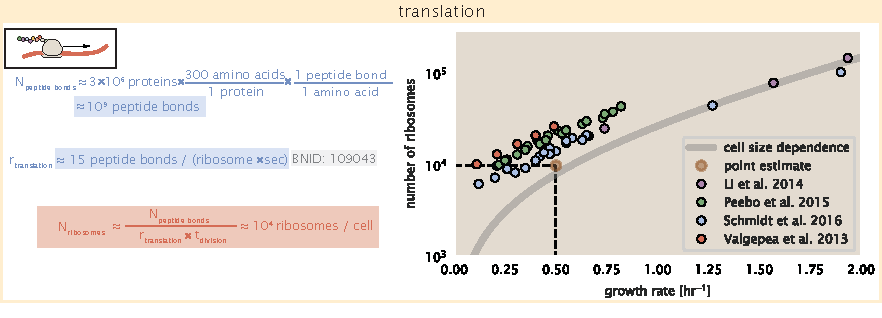
\includegraphics{main_figs/protein_synthesis_main.pdf}
    }
        \caption{\textbf{Estimation of the required number of ribosomes and the
        speed limit for bacterial replication.} (A) Estimation of the
        number of ribosomes required to synthesize 10$^9$ peptide bonds with an
        elongation rate of 15 peptide bonds per second. The
        average abundance of ribosomes is plotted as a function of growth rate.
        Our estimated values are shown for a growth rate of 0.5 hr$^{-1}$.
        Grey lines correspond to the estimated complex abundance calculated at
        different growth rates. (B) Estimation for the time to replicate a
        ribosome. This rate is independent of the number of ribosomes $R$ and instead is limited by the time required to
        double an individual ribosome.} \label{fig:protein_synthesis}

        \figsupp[Estimate and observed abundance and growth rate dependence
        of tRNA ligases.]{Estimation for the number of tRNA synthetases that
        will supply the required amino acid demand. The sum of all tRNA
        synthetases copy numbers are plotted as a function of growth rate
        ([ArgS], [CysS], [GlnS], [GltX], [IleS], [LeuS], [ValS], [AlaS]$_2$,
        [AsnS]$_2$, [AspS]$_2$, [TyrS]$_2$, [TrpS]$_2$, [ThrS]$_2$,
        [SerS]$_2$, [ProS]$_2$, [PheS]$_2$[PheT]$_2$, [MetG]$_2$,
        [lysS]$_2$, [HisS]$_2$, [GlyS]$_2$[GlyQ]$_2$).}{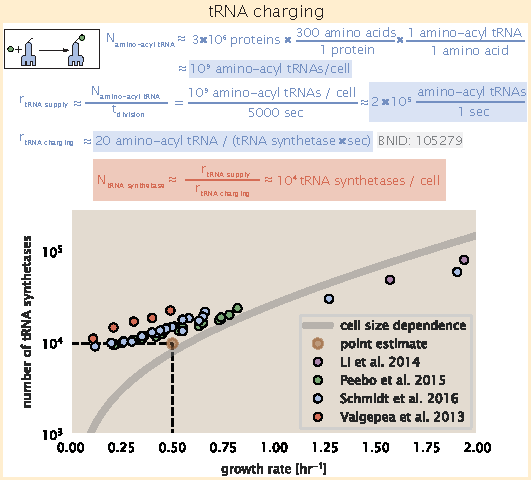
\includegraphics{main_figs/tRNA.pdf}}\label{figsupp:tRNA}
\end{figure}
